\documentclass[10pt,a4paper]{article}
\usepackage[utf8x]{inputenc}
\usepackage{ucs}
\usepackage{hyperref}
\usepackage{fancyhdr}
\usepackage{amsmath}
\usepackage{amsfonts}
\usepackage{graphicx}
\usepackage[frenchb]{babel}
\usepackage{amssymb}
\hypersetup{
pdfpagemode=UseOutlines,      % UseOutlines, UseThumbs, None, FullScreen : agencement au démarrage
pdfstartview=Fit,             % Fit, FitH, FitB, FitBH : vue de la page au départ (pleine largeur...)
pdffitwindow=true,            % bool: Maximiser
pdfpagelayout=TwoColumnsRight,% SinglePage, TwoColumnsRight/Left, OneColumn : affichage des pages
pdftoolbar=true,              % bool: Affichage de la barre d'outils
pdfmenubar=true,              % bool: Affichage de la barre de menus
bookmarksopen=false,          % bool: Dépliement des signets
bookmarksnumbered=true,       % bool: Numérotation des signets
colorlinks=true,              % bool: Liens colorés
pdfauthor={Beno\^it CARUSO & Jean-Baptiste LEPESME},     % Auteur
pdftitle={Rapport projet 10},    % Titre
pdfcreator=PDFLaTeX,          % 
pdfproducer=PDFLaTeX,         %
linkcolor=blue,               % Couleur des liens
urlcolor=blue,                %             url
anchorcolor=black,            %         du texte
citecolor=green,              % Couleur de citation 
frenchlinks=true,             % bool: Utiliser des petites majuscules pour les liens, plutôt que de la couleur
pdfborder={0 0 0}             % Ne pas encadrer les liens
}
\author{Benoît CARUSO & Jean-Baptiste LEPESME}
\title{Rapport projet 10}


\begin{document}
\maketitle

\section{Introduction}
	Le but de ce projet était de pouvoir contr\^oler un robot lego mindstorm à partir d'un smartphone sous Android.
	Ensuite il nous fallait utiliser LeJos pour pouvoir utiliser le robot comme un périphérique UpNp.
\section{Smartphone}
	L'application développée a été testée sur HTC Hero avec Android 2.1 (Eclair) et HTC Desire avec Android 2.2 (Froyo) et 2.3 (Gingerbread).
	Cette application devait permettre de récupérer les données des capteurs sur le smartphone pour ensuite communiquer avec le robot afin de le contr\^oler.
	Nous avons voulu que l'architecture de cette application soit orientée re-use et inspirée par les modèles à composants.
	Étant donné que les java beans ne peuvent pas s'utiliser sur Android nous avons opté pour une architecture plus classique.

	\subsection{Architecture}
	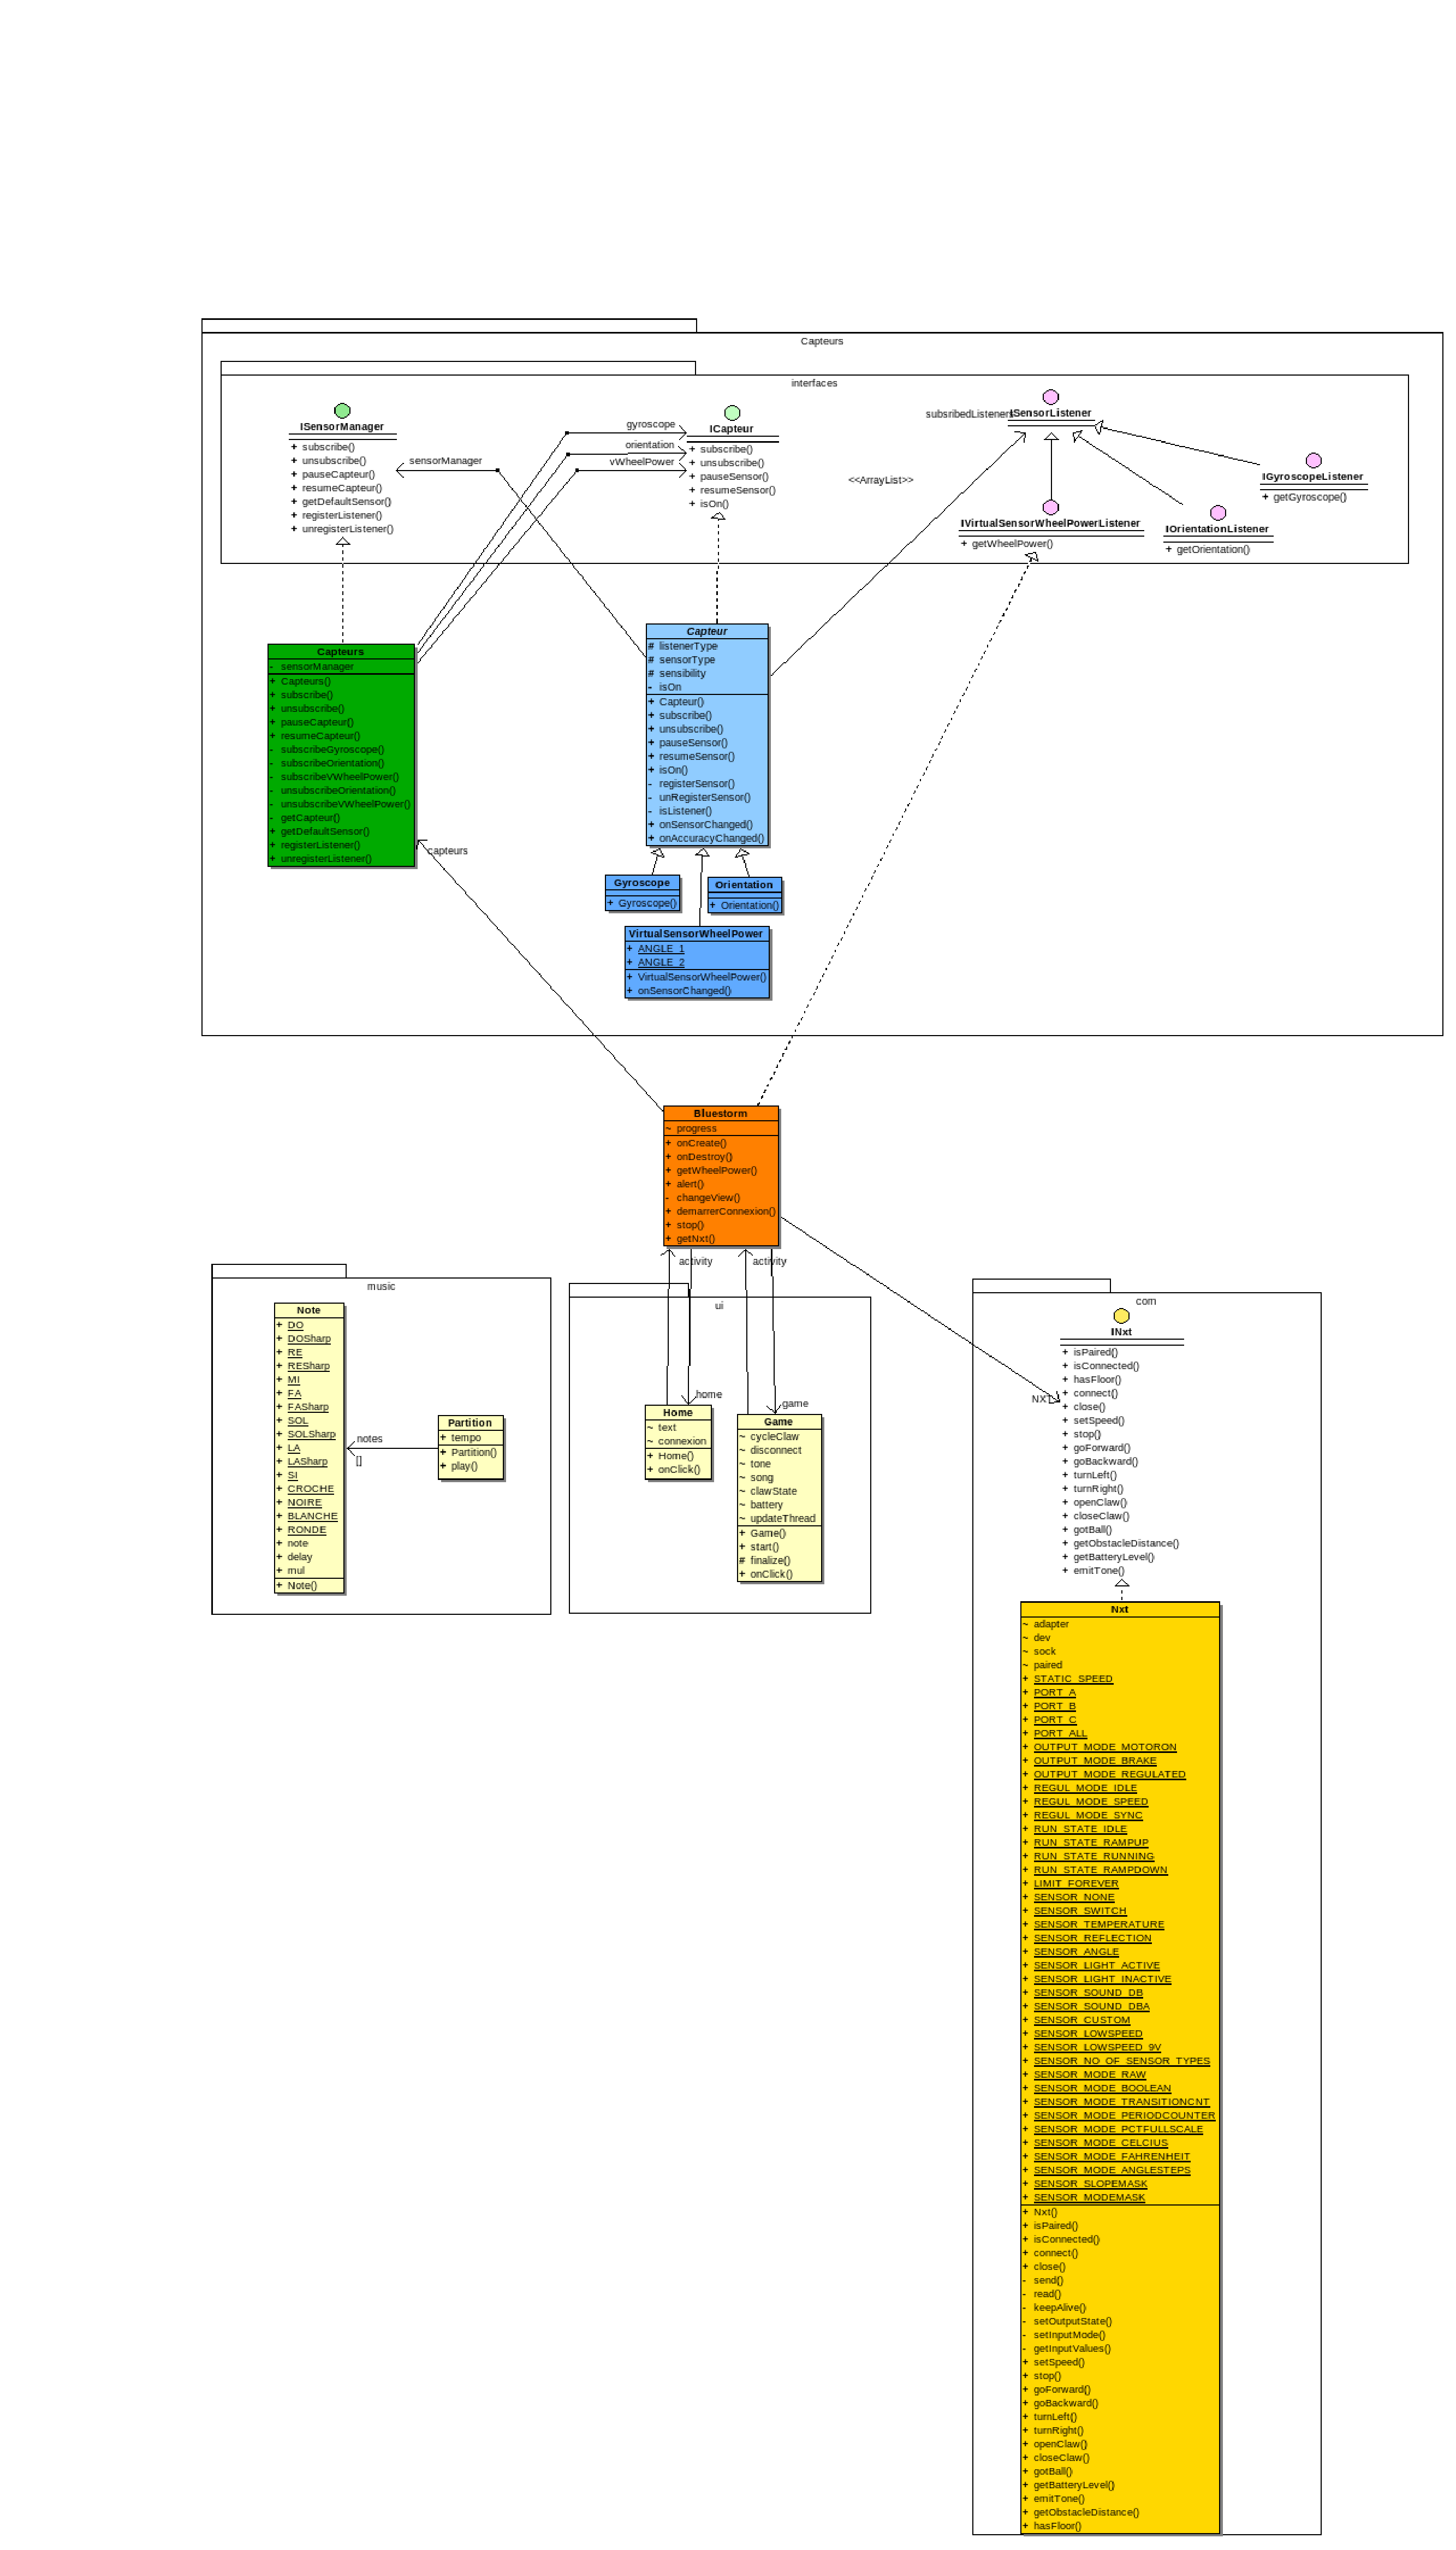
\includegraphics[width=15 cm]{diagramme.pdf} \\	
	
	\subsection{Capteurs}
	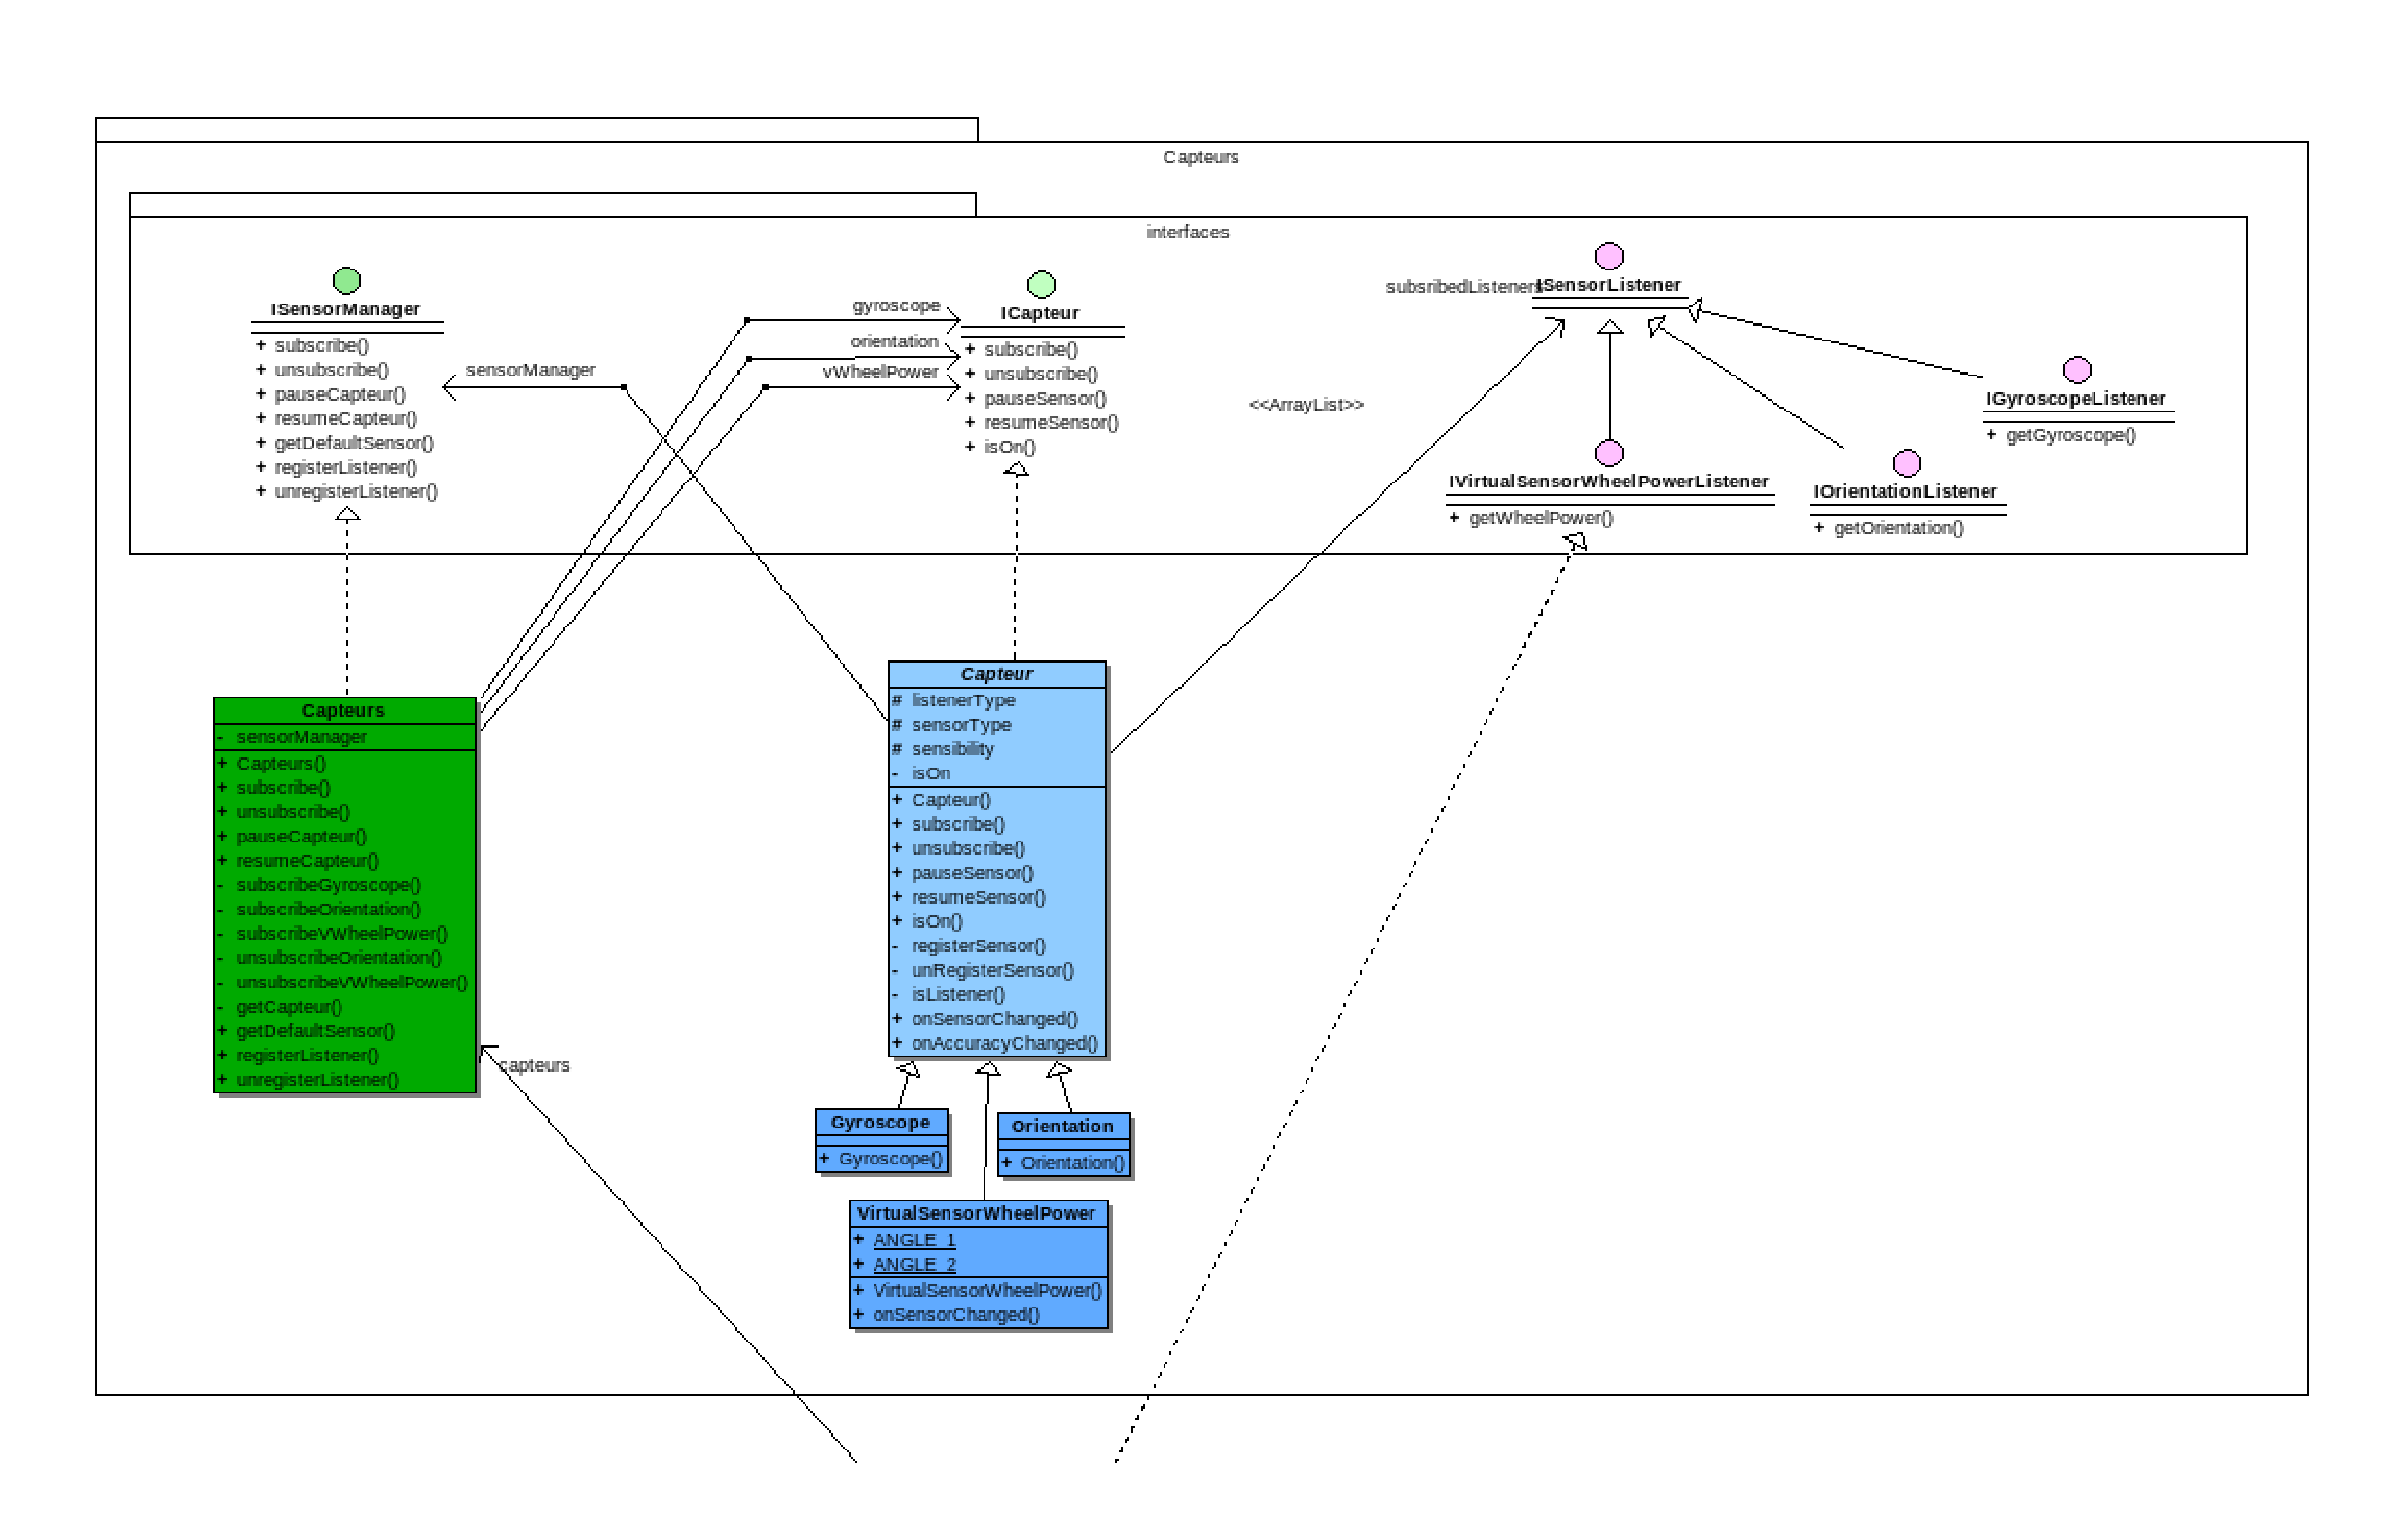
\includegraphics[width=15 cm]{diagramme1.pdf} \\
	
	\subsection{Communication}
	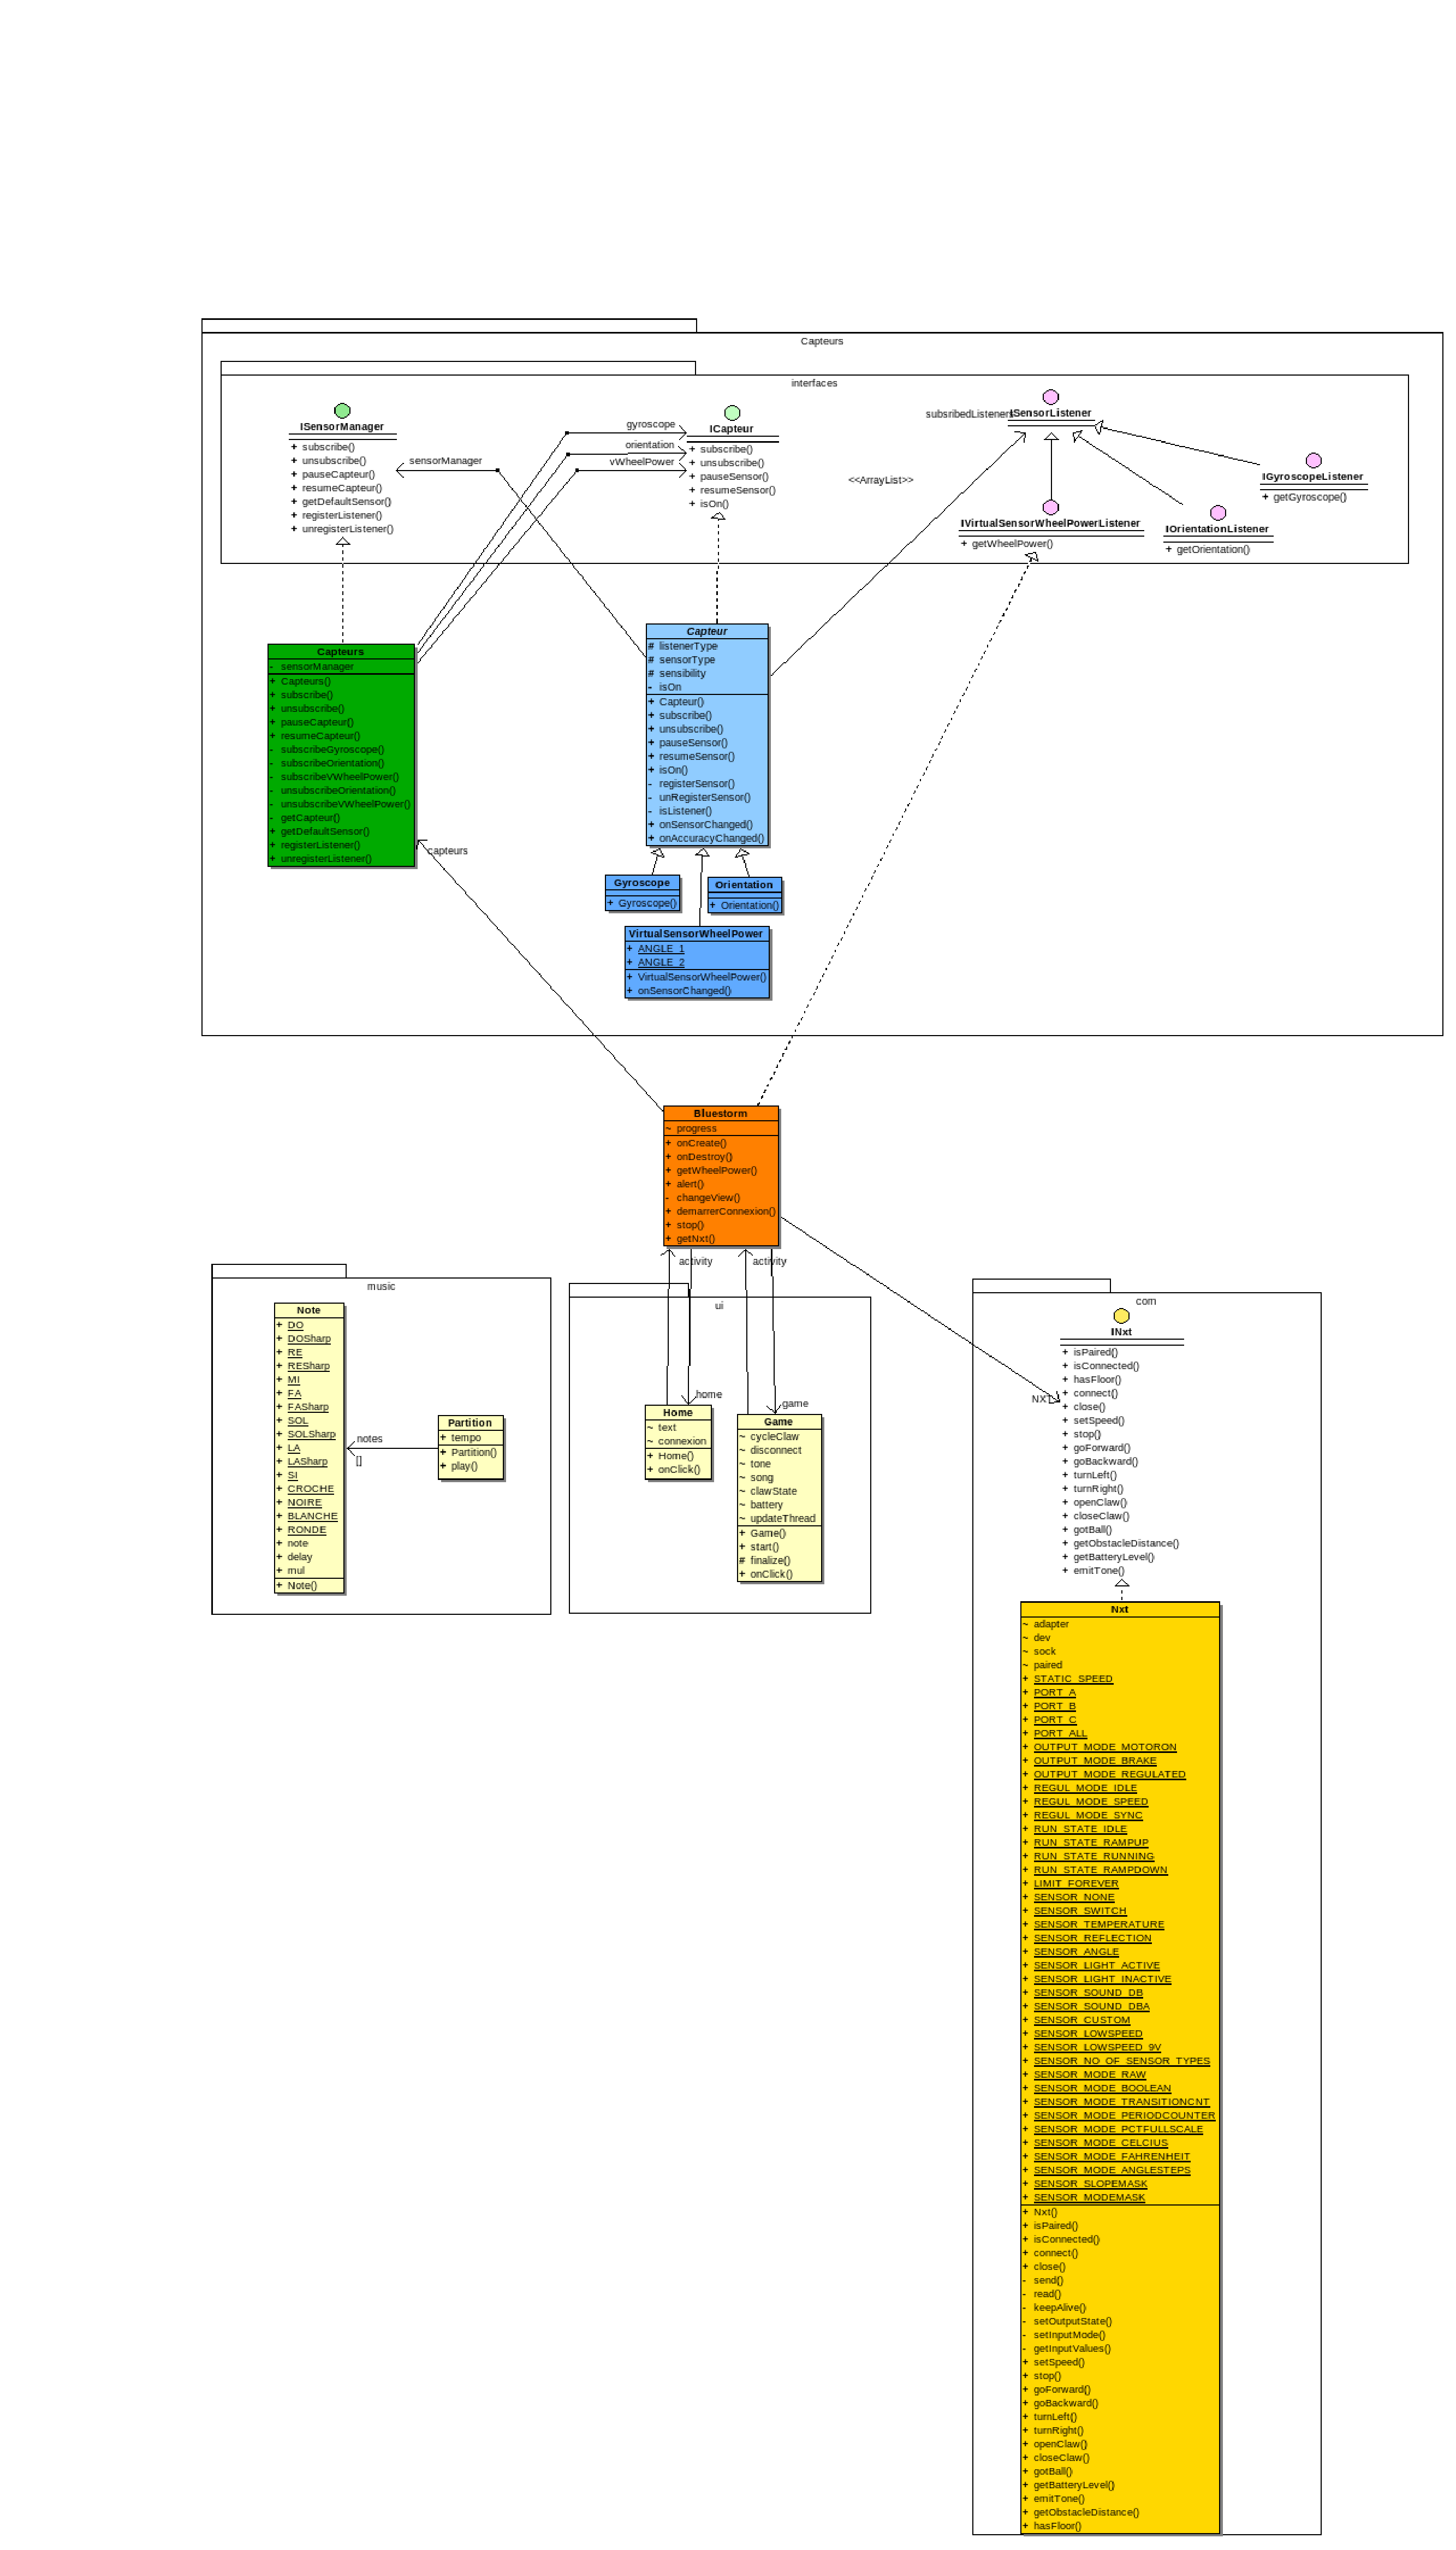
\includegraphics[width=15 cm]{diagramme.pdf} \\

\section{Robot}

\end{document}